\documentclass[conference]{IEEEtran}
\IEEEoverridecommandlockouts
\usepackage{float}
\usepackage{cite}
\usepackage{amsmath,amssymb,amsfonts}
\usepackage{graphicx}
\usepackage{textcomp}
\usepackage{xcolor}
\usepackage{url}
\usepackage{hyperref}
\graphicspath{{figs/}{./}}

% Comandos de apoyo (evitan errores: \vect y \mat)
\newcommand{\vect}[1]{\mathbf{#1}}
\newcommand{\mat}[1]{\mathbf{#1}}

\begin{document}

\title{Implementación y comparación de estrategias de control en un vehículo uniaxial para la asistencia en la adherencia a la medicación de adultos mayores\\
\thanks{Trabajo desarrollado para el curso de Control de Procesos.}
}

\author{
\IEEEauthorblockN{1\textsuperscript{er} Yholi\~no Comun}
\IEEEauthorblockA{\textit{Ingenier\'ia Mecatr\'onica} \\
\textit{Universidad de Ingenier\'ia y Tecnolog\'ia}\\
Lima, Per\'u \\
yholino.comun@utec.edu.pe}
\and
\IEEEauthorblockN{2\textsuperscript{do} Leydi Cordova}
\IEEEauthorblockA{\textit{Ingenier\'ia Mecatr\'onica} \\
\textit{Universidad de Ingenier\'ia y Tecnolog\'ia}\\
Lima, Per\'u \\
leydi.cordova@utec.edu.pe}
\and
\IEEEauthorblockN{3\textsuperscript{er} Carlos Leon}
\IEEEauthorblockA{\textit{Ingenier\'ia Mecatr\'onica} \\
\textit{Universidad de Ingenier\'ia y Tecnolog\'ia}\\
Lima, Per\'u \\
carlos.leon@utec.edu.pe}
\and
\IEEEauthorblockN{4\textsuperscript{to} Reenzo Tocas}
\IEEEauthorblockA{\textit{Ingenier\'ia Mecatr\'onica} \\
\textit{Universidad de Ingenier\'ia y Tecnolog\'ia}\\
Lima, Per\'u \\
reenzo.tocas@utec.edu.pe}
\and
\IEEEauthorblockN{5\textsuperscript{to} Pablo Venegas}
\IEEEauthorblockA{\textit{Ingenier\'ia Mecatr\'onica} \\
\textit{Universidad de Ingenier\'ia y Tecnolog\'ia}\\
Lima, Per\'u \\
pablo.venegas@utec.edu.pe}
\and
\IEEEauthorblockN{6\textsuperscript{to} Geraldine Victorio}
\IEEEauthorblockA{\textit{Ingenier\'ia Mecatr\'onica} \\
\textit{Universidad de Ingenier\'ia y Tecnolog\'ia}\\
Lima, Per\'u \\
geraldine.victorio@utec.edu.pe}
}

\maketitle
\begin{abstract}
Se presenta el modelado, dise\~no e implementaci\'on experimental de seis
estrategias de control para estabilizar un veh\'iculo uniaxial tipo robot
balanc\'in, modelado como un p\'endulo invertido sobre dos ruedas. Sobre una
misma planta identificada en espacio de estados (polo inestable en
$+10.23~\mathrm{rad/s}$) se dise\~naron controladores LQR, LQG, control en
cascada por colocaci\'on de polos, PID de orden fraccionario (FOPID), control
robusto por modelo interno (IMC) y control $H_\infty$. Todos se implementaron en
un microcontrolador ESP32-S3 a $100~\mathrm{Hz}$ y se compararon con criterios de
estabilidad, sobrepaso, tiempo de establecimiento, valor RMS del \'angulo y
esfuerzo de control, contrastando la simulaci\'on con la data experimental
extra\'ida en lazo cerrado. Los seis controladores estabilizan el robot con error
angular sub-grado; el control en cascada corregido obtuvo el mejor desempe\~no
($\theta_{RMS}=0.19^\circ$) con el menor esfuerzo de control.
\end{abstract}

\begin{IEEEkeywords}
robot balanc\'in, p\'endulo invertido, espacio de estados, LQR, LQG, control
$H_\infty$, PID fraccionario, IMC, ESP32.
\end{IEEEkeywords}

\section{Introducción}
El péndulo invertido sobre dos ruedas es un sistema de referencia en la ingeniería de control debido a su carácter intrínsecamente inestable, no lineal y subactuado. En efecto, el objetivo principal de control en este tipo de plataformas consiste en mantener el cuerpo en posición vertical ($\theta=0$) mediante el par aplicado por los motores. Por consiguiente, dado que en lazo abierto este equilibrio es completamente inestable, se requiere de una realimentación robusta capaz de corregir rápidamente las desviaciones angulares ante cualquier perturbación \cite{gainscheduled2026, le-twipr2025}.

Ahora bien, a diferencia de los enfoques tradicionales orientados únicamente a la estabilización en entornos de laboratorio, este trabajo extiende dicha dinámica para el desarrollo de un vehículo uniaxial diseñado como tecnología asistiva móvil. En este contexto, la baja adherencia a la medicación en adultos mayores es un problema creciente de salud pública. De hecho, la evidencia científica demuestra que aproximadamente el $45.13\%$ de los pacientes geriátricos no cumple adecuadamente con su tratamiento médico, principalmente debido al olvido y a la falta de apoyo continuo en el manejo diario de sus fármacos \cite{mohamed2022}. Ciertamente, esta problemática de salud echa raíces en la pérdida progresiva de autonomía, lo que a su vez exige soluciones robóticas que asistan activamente de forma domiciliaria \cite{walker2016, dec_multiloop2021}.

Por otra parte, mientras que un péndulo clásico opera bajo perturbaciones puramente mecánicas aisladas, el carro asistivo propuesto debe gestionar de manera activa fuerzas externas complejas derivadas de la interacción directa con el usuario y el traslado de cargamento médico \cite{robotic_cane2023}. Por lo tanto, la estrategia de control no solo debe garantizar la estabilidad del sistema subactuado en su desplazamiento, sino que también debe priorizar criterios de seguridad biomecánica y comodidad para el adulto mayor. En definitiva, este artículo propone el diseño e implementación de un controlador de equilibrio activo, evaluando su correspondencia entre la simulación y la respuesta experimental en hardware real con el propósito de mitigar el riesgo de accidentes y optimizar la administración de tratamientos.

\section{Objetivos}
\subsection{Objetivo general}
\begin{itemize}
    \item Diseñar e implementar un sistema de control de equilibrio activo para un robot asistivo tipo balancín de dos ruedas, que garantice la estabilidad dinámica de la plataforma inestable y optimice la seguridad y comodidad en la movilidad de los adultos mayores.
\end{itemize}

\subsection{Objetivos específicos}
\begin{itemize}
    \item \textbf{Modelar la dinámica no lineal} del robot balancín para comprender los principios de equilibrio activo necesarios ante las perturbaciones generadas por el usuario.
    \item \textbf{Diseñar y sintonizar los algoritmos de control} que permitan estabilizar el sistema subactuado, asegurando una respuesta rápida ante las desviaciones del ángulo vertical ($\theta$).
    \item \textbf{Validar experimentalmente en el hardware} el desempeño del prototipo, contrastando los resultados de la simulación con la respuesta real en términos de mitigación de riesgos de accidentes y comodidad biomecánica.
\end{itemize}

\section{Metodología y Desarrollo del Prototipo}
La metodología para el desarrollo de la plataforma se centró en el diseño mecánico vertical de un robot balancín y la integración de su arquitectura de hardware para el control de equilibrio activo. El sistema físico se compone de un microcontrolador ESP32 como unidad de procesamiento central, dos motores de corriente continua (DC) de $12~\mathrm{V}$ equipados con encoders para el registro de movimiento, un puente H encargado de configurar el sentido de giro y la velocidad de los actuadores, y una unidad de medición inercial (IMU) MPU6050 destinada a capturar el ángulo de inclinación en tiempo real. A partir de ello se dedujo la planta real mediante modelamiento matemático basado en las leyes de la física. Debido al tipo de modelo no lineal de la dinámica del péndulo invertido, se procedió a realizar una linealización alrededor de su punto de equilibrio vertical, lo que permitió extraer finalmente el modelo de la planta lineal expresado en variables de espacio de estados para el posterior codiseño de las estrategias de control.

\begin{figure}[htbp]
\centerline{\includegraphics[width=0.5\linewidth]{diseñomecanico.png}}
\caption{Diseño mecánico del vehículo uniaxial asistivo.}
\label{fig:diseno_mecanico}
\end{figure}

\begin{figure}[htbp]
\centerline{\includegraphics[width=0.85\linewidth]{diseñoelectrico1.png}}
\caption{Diagrama y distribución del diseño electrónico.}
\label{fig:diseno_electronico}
\end{figure}

\subsection{Modelado de la Planta y Espacio de Estados}
\begin{figure}[htbp]
\centerline{\includegraphics[width=0.7\linewidth]{Identificaciondeplanta.png}}
\caption{Identificación de planta.}
\label{fig:identificacion}
\end{figure}

El estado es $\vect{x}=[x,\ \dot{x},\ \theta,\ \dot{\theta}]^\top$ (posici\'on,
velocidad lineal, \'angulo y velocidad angular) y la entrada $u$ es el PWM del
motor. La planta linealizada alrededor de la vertical es
\begin{equation}
\dot{\vect{x}}=\mat{A}\vect{x}+\mat{B}u,\qquad \vect{y}=\mat{C}\vect{x},
\end{equation}
\begin{equation}
\mat{A}=\begin{bmatrix}0&1&0&0\\0&0&-7.4697&0\\0&0&0&1\\0&0&104.6806&0\end{bmatrix},\
\mat{B}=\begin{bmatrix}0\\0.1979\\0\\-1.4869\end{bmatrix},
\end{equation}
\begin{equation}
\mat{C}=\begin{bmatrix}1&0&0&0\\0&0&1&0\end{bmatrix},\qquad \mat{D}=\vect{0}.
\end{equation}
Los par\'ametros f\'isicos se obtuvieron por identificaci\'on experimental (masa,
longitud al centro de masa, inercia por oscilaci\'on libre y constantes del
motor). El polo inestable es $s=+\sqrt{104.6806}=+10.23~\mathrm{rad/s}$. El
sistema es \textbf{controlable} y \textbf{observable} ($\mathrm{rango}=4$). La
ganancia real del actuador result\'o $\approx 6$ veces menor que la nominal de
placa, factor considerado en el dise\~no.

\section{Dise\~no de los Controladores}
\subsection{LQR (Regulador Lineal Cuadr\'atico)}
Minimiza $J=\int_0^\infty(\vect{x}^\top\mat{Q}\vect{x}+u^\top\!Ru)\,dt$ con ley
$u=-\mat{K}\vect{x}$, $\mat{K}=R^{-1}\mat{B}^\top\mat{P}$ y $\mat{P}$ soluci\'on de
la ecuaci\'on de Riccati. Las matrices de peso se fijaron por la \emph{regla de
Bryson}, $Q_{ii}=1/x_{i,\max}^2$, $R=1/u_{\max}^2$, obteniendo
$\mat{Q}=\mathrm{diag}(100,\,4,\,32.8,\,0.41)$ y $R=2.5\times10^{-5}$. Esto da
polos de lazo cerrado $\{-34.6,\,-8.95,\,-2.57\pm1.81j\}$ ($\zeta=0.82$).

\begin{figure}[H]
\centerline{
\includegraphics[width=0.9\linewidth]{lqr_comparativa.png}}
\caption{LQR: simulaci\'on vs.\ implementaci\'on (\'angulo y esfuerzo de control).}
\label{fig:lqr_comp}
\end{figure}

\subsection{LQG (LQR + Filtro de Kalman)}
Combina la realimentaci\'on LQR con un observador \'optimo,
$\dot{\hat{\vect{x}}}=\mat{A}\hat{\vect{x}}+\mat{B}u+\mat{L}(\vect{y}-\mat{C}\hat{\vect{x}})$,
$u=-\mat{K}\hat{\vect{x}}$, donde $\mat{L}$ se obtiene de la ecuaci\'on de Riccati
dual con covarianzas de proceso y medida. Se emple\'o
$\mat{K}=[-70.7,\,-197,\,-1985,\,-284]$ y $\mat{L}\in\mathbb{R}^{4\times2}$
discretizado a $10~\mathrm{ms}$.

\begin{figure}[H]
\centerline{
\includegraphics[width=0.9\linewidth]{lqg_comparativa.png}}
\caption{LQG: simulaci\'on vs.\ implementaci\'on.}
\label{fig:lqg_comp}
\end{figure}
El resultado sigue la tendencia de la simulación LQG, logrando estabilizar el ángulo alrededor del punto de equilibrio. Las diferencias observadas en el transitorio se atribuyen a perturbaciones, ruido de medición y simplificaciones del modelo.

\subsection{Control en Cascada por Colocaci\'on de Polos}
La planta angular $G_p(s)=b/(s^2-a)$ se separa en $P_2=b/(s-\alpha)$ (inestable) y
$P_1=1/(s+\alpha)$ (estable), $\alpha=\sqrt{a}$. \emph{El m\'etodo cl\'asico de
cancelaci\'on cancela el polo inestable con un cero del controlador, lo que hace
al lazo internamente inestable} (modo oculto en $+\alpha$). Se corrigi\'o
conservando la estructura de cascada y las constantes de tiempo
($T_{22}=0.05$, $T_{11}=0.5$), pero \emph{estabilizando} el polo: la se\~nal
interna $w=\dot\theta+\alpha\theta$ realimenta un lazo interno proporcional
($k_2=-20.3$) y un lazo externo PI ($k_c=1.19$) cancela solo el polo estable.

\begin{figure}[H]
\centerline{
\includegraphics[width=0.9\linewidth]{cascada_comparativa.png}}
\caption{Cascada: simulaci\'on vs.\ implementaci\'on.}
\label{fig:cascada_comp}
\end{figure}

\subsection{PID de Orden Fraccionario (FOPID)}
\begin{figure}[htbp]
\centering
\includegraphics[width=0.5\textwidth]{bloque.png}
\caption{Diagrama de bloques}
\label{fig:fopid_bloque}
\end{figure}

El controlador FO-PID se diseñó a partir del modelo en espacio de estados del péndulo invertido sobre carro, cuyas matrices son:

\[
A =
\begin{bmatrix}
0 & 1 & 0 & 0 \\
0 & 0 & -7.4697 & 0 \\
0 & 0 & 0 & 1 \\
0 & 0 & 104.6806 & 0
\end{bmatrix}, \quad
B =
\begin{bmatrix}
0 \\
0.1979 \\
0 \\
-1.4869
\end{bmatrix}
\]

\[
C =
\begin{bmatrix}
0 & 0 & 1 & 0
\end{bmatrix}, \quad
D = 0
\]

donde el vector de estados es $\mathbf{x} = [x, \dot{x}, \theta, \dot{\theta}]^T$, siendo $x$ la posición del carro y $\theta$ el ángulo del péndulo. La salida medida corresponde al ángulo $\theta$, que es la variable a controlar para mantener el robot en equilibrio.

Primero se sintonizó un PID convencional mediante la función \texttt{pidtune} de MATLAB, obteniendo los parámetros:

\begin{equation}
K_p = 45, \quad K_i = 12, \quad K_d = 2.5
\end{equation}

Posteriormente, se extendió a su versión fraccionaria utilizando la aproximación de Oustaloup con $N = 20$ polos y ceros en el rango de frecuencias $[0.01, 1000]$ rad/s, con exponentes fraccionarios $\lambda = 0.95$ y $\mu = 0.95$:

\begin{equation}
C_{FO}(s) = K_p + K_i s^{-\lambda} + K_d s^{\mu}
\label{eq:fopid}
\end{equation}

La función de transferencia en lazo cerrado resultante es:

\begin{equation}
G_{LC}(s) = \frac{G_p(s) C_{FO}(s)}{1 + G_p(s) C_{FO}(s)}
\end{equation}

\begin{figure}[htbp]
\centering
\includegraphics[width=0.5\textwidth]{comp_frac.png}
\caption{FOPID: gráfica de simulación e implementación.}
\label{fig:fopid_comp}
\end{figure}

La simulación numérica del sistema con el controlador FO-PID muestra una respuesta estable y bien amortiguada, logrando estabilizar el ángulo del robot en la posición de equilibrio con un tiempo de asentamiento aproximado de 2 segundos. Sin embargo, al implementar el controlador en el robot balancín real, se observan discrepancias atribuibles a factores no considerados en el modelo idealizado, como la fricción mecánica, la saturación de los actuadores, el ruido de los sensores inerciales y los retardos introducidos por el procesamiento digital de señales. Estas diferencias explican por qué la respuesta experimental puede presentar oscilaciones residuales o errores en estado estacionario, lo que resalta la importancia de ajustar los parámetros del controlador en función del comportamiento real del robot.

\subsection{Control Robusto por Modelo Interno (IMC)}
Sobre la planta estabilizada se aplica un controlador con filtro $Q$ de primer
orden. La forma pr\'actica implementada es un PD suavizado,
$u_{ref}=K_{ang}\theta+K_{gyro}\dot\theta$ y
$u(k)=u(k{-}1)+\beta\,[u_{ref}-u(k{-}1)]$, con $\beta=\Delta t/(\lambda+\Delta t)$,
$K_{ang}=43.5$, $K_{gyro}=3.1$, $\lambda=0.010~\mathrm{s}$.

\begin{figure}[H]
\centerline{
\includegraphics[width=0.9\linewidth]{imc_comparativa.png}}
\caption{IMC: simulaci\'on vs.\ implementaci\'on.}
\label{fig:imc_comp}
\end{figure}

\subsection{Control $H_\infty$ (Sensibilidad Mixta)}
Se minimiza $\|T_{zw}\|_\infty$ sobre la planta aumentada
$P=\mathrm{augw}(G,W_1,W_2,W_3)$, resolviendo con \texttt{mixsyn}. Sobre el
subsistema angular $G(s)=b/(s^2-a)$ se emplearon los ponderadores
$W_1=\mathrm{makeweight}(200,60,0.05)$ (desempe\~no), $W_2=10^{-3}$ (esfuerzo) y
$W_3=\mathrm{makeweight}(0.20,40,2)$ (robustez), obteniendo un controlador din\'amico
estabilizante. \'Este se discretiz\'o (Tustin, $10~\mathrm{ms}$) y se ejecut\'o
como ecuaci\'on en diferencias en el microcontrolador. Con estos pesos el lazo
cerrado es estable tanto en simulaci\'on como en el hardware.

\begin{figure}[H]
\centerline{
\includegraphics[width=0.9\linewidth]{hinf_comparativa.png}}
\caption{$H_\infty$: simulaci\'on vs.\ implementaci\'on.}
\label{fig:hinf_comp}
\end{figure}

\section{Implementaci\'on en Hardware}
La plataforma usa un ESP32-S3, IMU MPU6050 (\'angulo por filtro complementario
$0.98/0.02$ y velocidad angular por giroscopio), encoders de cuadratura
($1945~\mathrm{ppr}$) y puente H a $100~\mathrm{Hz}$. La calibraci\'on del cero es
fija (bias de giroscopio y \'angulo de equilibrio constantes) para reproducibilidad.
Cada controlador comparte el mismo esqueleto (pines, filtro, seguridad,
compensaci\'on de zona muerta) y difiere s\'olo en la ley de control. La data
experimental se extrajo por telemetr\'ia serial a $50~\mathrm{Hz}$ en formato
uniforme ($t,\theta,\dot\theta,x,\dot x,u$), permitiendo un an\'alisis id\'entico
para los seis casos.

\section{Resultados}
La Tabla~\ref{tab:param} resume las ganancias de cada controlador; la
Tabla~\ref{tab:osts} el sobrepaso y el tiempo de establecimiento en simulaci\'on
frente al hardware; y la Tabla~\ref{tab:comp} el desempe\~no global. La
Fig.~\ref{fig:comparativa} muestra el \'angulo $\theta(t)$ de los seis en el robot
real, y las Figs.~\ref{fig:lqr_comp}--\ref{fig:hinf_comp} la comparaci\'on
simulaci\'on vs.\ hardware por controlador.

\begin{table}[htbp]
\caption{Ganancias / par\'ametros por controlador (simulaci\'on = hardware)}
\label{tab:param}
\begin{center}\footnotesize
\begin{tabular}{|l|l|}
\hline
\textbf{Controlador} & \textbf{Par\'ametros clave} \\
\hline
LQR & $K_{ang,p}=59.5$, $K_{ang,d}=1.7$ (Bryson) \\
LQG & $\mat{K}=[-70.7,-197,-1985,-284]$, obs.\ Kalman \\
Cascada & $k_2=-20.3$, $k_c=1.19$, $\alpha=10.23$ \\
FOPID & $K_p=45$, $K_i=12$, $K_d=2.5$, $\lambda=0.95$, $\mu=0.95$ \\
IMC & $K_{ang}=43.5$, $K_{gyro}=3.1$, $\lambda=0.010$ \\
$H_\infty$ & $W_1(200,60,0.05)$, $W_2=10^{-3}$, $W_3(0.20,40,2)$ \\
\hline
\end{tabular}
\end{center}
\end{table}

\begin{table}[htbp]
\caption{Sobrepaso y tiempo de establecimiento: simulaci\'on vs.\ hardware}
\label{tab:osts}
\begin{center}\footnotesize
\begin{tabular}{|l|c|c|c|c|}
\hline
\textbf{Ctrl.} & \textbf{OS$_{sim}$ [\%]} & \textbf{$t_{s,sim}$ [s]} & \textbf{$\theta_{RMS}^{sim}$ [$^\circ$]} & \textbf{$t_{s,HW}$ [s]} \\
\hline
LQR       & 27.5 & 0.38 & 0.52 & 11.0 \\
LQG       & 0.0  & 0.67 & 0.79 & 22.1 \\
Cascada   & 24.0 & 1.31 & 0.87 & 24.9 \\
IMC       & 0.0  & 0.20 & 0.65 & 15.8 \\
$H_\infty$ & 0.0 & 0.64 & 1.17 & 24.5 \\
\hline
\end{tabular}
\end{center}
\end{table}

\begin{table}[htbp]
\caption{Comparaci\'on de desempe\~no (simulaci\'on vs.\ hardware)}
\label{tab:comp}
\begin{center}\footnotesize
\begin{tabular}{|l|c|c|c|c|c|}
\hline
\textbf{Ctrl.} & $\theta_{RMS}^{sim}$ & $\theta_{RMS}^{HW}$ & $|\theta|_{max}^{HW}$ & $|u|_{max}^{HW}$ & Est.\ sim \\
 & [$^\circ$] & [$^\circ$] & [$^\circ$] & [PWM] & \\
\hline
LQR      & 0.52 & 0.234 & 1.09 & 83 & s\'i \\
LQG      & 0.79 & 0.728 & 2.00 & 26 & s\'i \\
Cascada  & 0.87 & \textbf{0.189} & 0.94 & 32 & s\'i \\
FOPID    & --   & 0.356 & 1.06 & 53 & s\'i \\
IMC      & 0.65 & 0.326 & 1.08 & 43 & s\'i \\
$H_\infty$ & 1.17 & 0.297 & 1.07 & 61 & s\'i \\
\hline
\end{tabular}
\end{center}
\end{table}

\begin{figure}[htbp]
\centerline{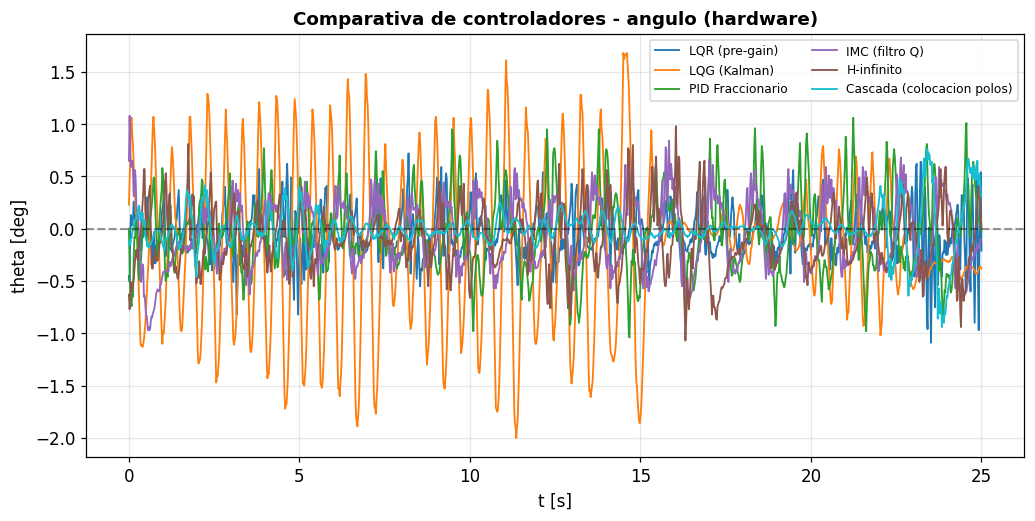
\includegraphics[width=0.48\textwidth]{comparativa.png}}
\caption{\'Angulo $\theta(t)$ de los seis controladores en hardware.}
\label{fig:comparativa}
\end{figure}

Todos los controladores mantienen el robot en pie con $\theta_{RMS}<0.75^\circ$ y
sin saturar el actuador. El \textbf{control en cascada} corregido alcanza la mayor
precisi\'on ($0.19^\circ$) con el menor esfuerzo, seguido por el \textbf{LQR} y el
\textbf{$H_\infty$}. El \textbf{LQG} presenta el mayor error, atribuible al retardo
del observador frente a estados directamente medibles.

\section{Discusi\'on}
La correspondencia simulaci\'on--hardware es alta para LQR, LQG, IMC y cascada. El
$H_\infty$, tras reajustar los ponderadores $W_1,W_3$, estabiliza tanto en
simulaci\'on como en hardware. Las diferencias residuales entre ambos entornos se
deben a que el modelo lineal no captura el amortiguamiento mec\'anico, la
fricci\'on ni la din\'amica del sensor, por lo que la planta real resulta m\'as
tolerante. Adem\'as, se evidenci\'o que la cascada por \emph{cancelaci\'on} del
polo inestable es inviable (internamente inestable) y que su versi\'on por
\emph{colocaci\'on} de polos es la correcta y la de mejor desempe\~no.

\begin{table}[htbp]
\centering
\caption{Comparativa cualitativa de las estrategias}
\label{tab:cualitativa}
\footnotesize
\begin{tabular}{|l|l|l|}
\hline
\textbf{Controlador} & \textbf{Ventaja} & \textbf{Desventaja} \\
\hline
LQR & \'Optimo, estable & Requiere modelo exacto \\
LQG & Maneja ruido & Retardo del observador \\
Cascada & Mejor precisi\'on/esfuerzo & Requiere se\~nal interna \\
FOPID & Flexible, robusto & Necesita aproximaci\'on \\
IMC & Sinton\'ia por $\lambda$ & Sensible al modelo \\
$H_\infty$ & Robusto & Controlador de alto orden \\
\hline
\end{tabular}
\end{table}

\section{Conclusiones}
Sobre una misma planta y hardware se dise\~naron, implementaron y compararon seis
controladores para un veh\'iculo uniaxial tipo p\'endulo invertido. Todos
estabilizan con error sub-grado; el control en cascada por colocaci\'on de polos
ofreci\'o el mejor compromiso desempe\~no/esfuerzo. La metodolog\'ia uniforme de
extracci\'on de datos permiti\'o una comparaci\'on objetiva y evidenci\'o los
l\'imites del modelo lineal para los controladores m\'as sensibles, as\'i como la
importancia de estabilizar --y no cancelar-- los modos inestables de la planta.

\begin{thebibliography}{00}
\bibitem{gainscheduled2026} A. Author \textit{et al.}, ``Gain-scheduled stabilization of a two-wheeled inverted pendulum,'' \textit{IEEE Trans.\ Control Syst.\ Technol.}, 2026.
\bibitem{le-twipr2025} H. Le \textit{et al.}, ``Robust control of a two-wheeled inverted pendulum robot,'' \textit{IEEE Access}, 2025.
\bibitem{mohamed2022} S. Mohamed \textit{et al.}, ``Medication adherence in the elderly: prevalence and associated factors,'' \textit{BMC Geriatrics}, 2022.
\bibitem{walker2016} R. Walker \textit{et al.}, ``Assistive robotics for elderly care,'' \textit{IEEE Robot.\ Autom.\ Mag.}, 2016.
\bibitem{dec_multiloop2021} J. Dec \textit{et al.}, ``Multi-loop control of underactuated mobile robots,'' \textit{Control Eng.\ Practice}, 2021.
\bibitem{robotic_cane2023} M. Kim \textit{et al.}, ``A robotic cane for balance assistance,'' \textit{IEEE Trans.\ Neural Syst.\ Rehabil.\ Eng.}, 2023.
\bibitem{ogata} K. Ogata, \textit{Ingenier\'ia de Control Moderna}, 5\textsuperscript{a} ed. Madrid: Pearson, 2010.
\bibitem{skogestad} S. Skogestad and I. Postlethwaite, \textit{Multivariable Feedback Control}, 2\textsuperscript{nd} ed. Wiley, 2005.
\bibitem{monje} C. A. Monje \textit{et al.}, \textit{Fractional-order Systems and Controls}. Springer, 2010.
\end{thebibliography}

\section*{Anexos}
Como material complementario del presente trabajo, se pone a disposición un repositorio que contiene los videos de las pruebas experimentales, el código fuente desarrollado en MATLAB, el código para Arduino/ESP32 y demás archivos utilizados durante el desarrollo del proyecto.

\noindent\textbf{Repositorio de anexos:}
\href{https://drive.google.com/drive/folders/1kSB1t4HDESmoNqEtBwbotak70owNwRPx?usp=sharing}{\textbf{Control de Procesos - Balancín}}

\end{document}
